\section{Wireframes}
\label{sec:wireframes}

  \subsection{Design choices}
    \begin{wrapfigure}{l}{0.35\textwidth}
      \centering
      \vspace{-5pt}
      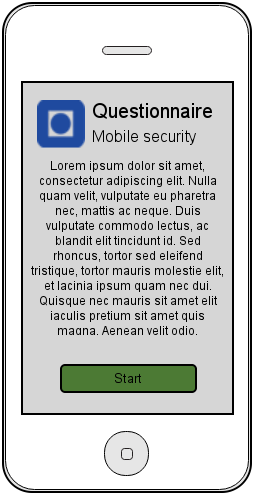
\includegraphics[scale=0.40]{screens/v3/mobile/mobile1-1.png}
      \caption{Introduction}
      \label{fig:wireframe1}
    \end{wrapfigure}
    
  In this section, there will be a description of how to build a system for data collection. The questionnaire will be created as a web application that will be easy to distribute over the Internet. In this report, the design of the system will be described in detail. The implementation will be finished next semester and will, therefore, not be a product included in this project. During this project, I have spent much time designing the look of the system, as well as the structure. The respondents are going to answer the questionnaire on a smartphone; there is many usability requirements that must be considered. First, the system must be easy to learn. When the system should be easy to learn, the respondents should be familiar with icons and elements used in order to be able to complete the questionnaire. Second, the systems should be efficient. When answering on a mobile phone, this should be considered as essential requirements to fulfill. If the questionnaire takes too long time, it is possible that many people will not complete or even want to start.

  To support efficiency, there is added images that easily can be interpreted. Even if the respondent is not fluent in English, the respondent should be able to understand the questions by looking at the icons used. At this point, it is not decided if it is needed to add support for other languages. There is going to be conducted two pilot tests of the wireframes to ensure the two selected usability attributes learnability and efficiency. The first test will focus on the time used for completion of the questionnaire, and the other test will remove the questions in order to test if the icons is understandable. The test will further be described in Section~\ref{sec:pretest}. The new test will be conducted when the system is implemented, and will be carried out and documented next semester.



  \todo{Legge til kilder på usability}
  \todo{What is a wireframe?}

  Figure~\ref{fig:wireframe1} is the first screen that the respondents meet when they access the questionnaire. This includes a description of the research, information about the questionnaire, and privacy concerns. This is the first part that the respondents meet, so it is important that the respondent feel confident. The contact information provides a creditability to the questionnaire, so the respondents can feel save that information is handled correctly accordingly to the information that is given. It also allows the respondents to ask questions if they have any questions or want to Google the researcher sending out the questionnaire. A questionnaire asking for personal information might seem scary for some respondents, it is then comforting to be able to see who this person is.

  When the respondents are decided to participate, they press start and is transferred to the screen in Figure~\ref{fig:wireframe2}. This screen is providing information about the Android Unlock Patten, so they can know how to type the pattern. If the respondents have not tried the unlock pattern before, they will get the choice to try the scheme before entering their pattern. For experienced users, they can skip the training for saving time. Figure~\ref{fig:wireframe3} shows the training mode. The registered patterns are collected to be able to compare the pattern in the training mode, as well as the selected patterns. Figure~\ref{fig:wireframe4} is the start screen for the pattern creation. The respondents are asked to make three patterns, one for a shopping account, one pattern for their smartphone, and one pattern for their banking account.

    \begin{figure}[H]
      \subfigure[Introduction to Android Lock Pattern]{
        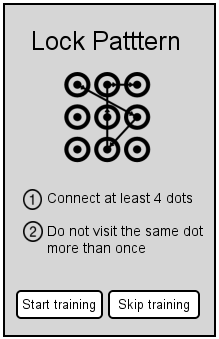
\includegraphics[scale=0.48]{screens/v3/plain/plain1-2.png}
        \label{fig:wireframe2}
      }
      \subfigure[Training mode]{ 
        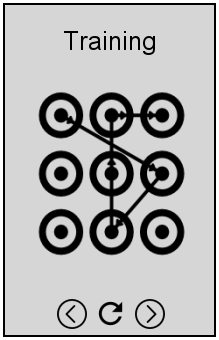
\includegraphics[scale=0.48]{screens/v3/plain/plain1-3.png}
        \label{fig:wireframe3}
      }
      \subfigure[Introduction to pattern creation]{
        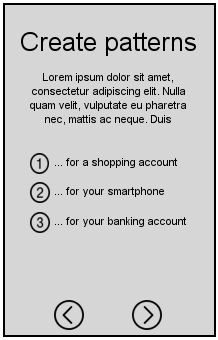
\includegraphics[scale=0.48]{screens/v3/plain/plain1-4.png}
        \label{fig:wireframe4}
      }
    \end{figure}

  The pattern creation is showed in Figure~\ref{fig:wireframe5}, Figure~\ref{fig:wireframe6}, and Figure~\ref{fig:wireframe7}. For different users, the order of the different pattern will occur in a different order using the Latin Square method that was described in Section~\ref{sec:layout}.

    \begin{figure}[H]
      \subfigure[Creation of pattern 1]{
        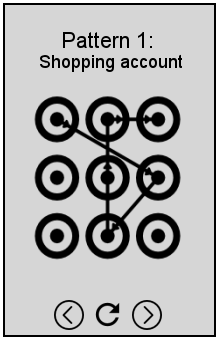
\includegraphics[scale=0.48]{screens/v3/plain/plain1-5.png}
        \label{fig:wireframe5}
      }
      \subfigure[Creation of pattern 2]{
        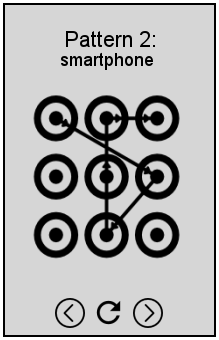
\includegraphics[scale=0.48]{screens/v3/plain/plain1-6.png}
        \label{fig:wireframe6}
      }
      \subfigure[Creation of pattern 3]{
        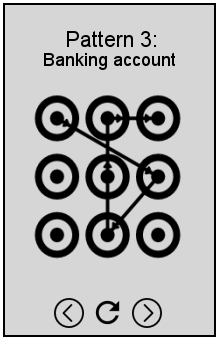
\includegraphics[scale=0.48]{screens/v3/plain/plain1-7.png}
        \label{fig:wireframe7}
      }
    \end{figure}

  The first part have focused on the pattern creation because it is the most crucial information needed. After the pattern creation, the questionnaire will now ask the respondents about demographic, experience and use of lock screens and some information about the device used to answer the questionnaire. All of these questions is found in Table~\ref{tab:questions}, and most of the human properties is found in the analysis of human properties in Section~\ref{sec:datarequirements}.

  Figure~\ref{fig:wireframe8} is asking about the respondent's hand size. The answers from this question will be subjective, but there is not any other way this can be asked. Asking people to measure the actual size would be preferable but would require too much time for the respondents. They also might not have any instruments available to measure their precise length. Figure~\ref{fig:wireframe9} is asking the respondents about their screen size. This will also be subjective. In order to be able to get the correct size, there will be used JavaScript to detect the actual size of the screen in (illustrated in Listing~\ref{list:screen}). Why add a question that is possible to detect automatically? It is not desired to collect data that is not explicitly asked.

  \medskip
  \begin{lstlisting}[caption=Detecting screen size in JavaScript, label=list:screen]
    var height = window.screen.availHeight;
    var width = window.screen.availWidth;
  \end{lstlisting}

  In Figure~\ref{fig:wireframe10} it is asked for the hand used when the respondent answered the questionnaire. This can be used when predicting the likely initial starting point that was discussed in Section~\ref{sec:datarequirements}

    \begin{figure}[H]
    \ContinuedFloat
      \subfigure[Q1: Hand size]{
        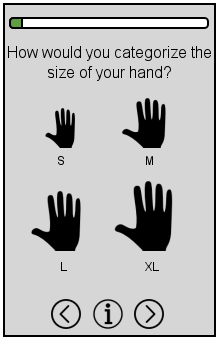
\includegraphics[scale=0.48]{screens/v3/plain/plain2-1.png}
        \label{fig:wireframe8}
      }
      \subfigure[Q2: Screen size]{
        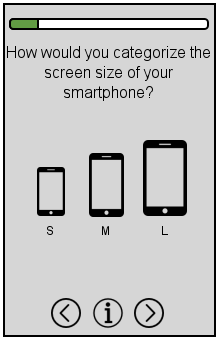
\includegraphics[scale=0.48]{screens/v3/plain/plain2-2.png}
        \label{fig:wireframe9}
      }
      \subfigure[Q3: Handedness]{
        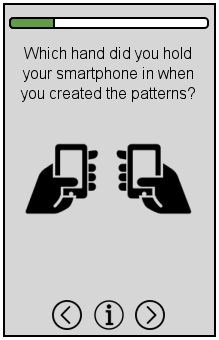
\includegraphics[scale=0.48]{screens/v3/plain/plain2-3.png}
        \label{fig:wireframe10}
      }
    \end{figure}

    When the respondent is using either left- or right-hand, it is crucial to know the finger used (Figure~\ref{fig:wireframe11}). If the respondent is using their thumb, it is likely that they held the smartphone in one hand. If the forefinger is used, it is likely that the respondent used the forefinger. My hypothesis is that this is necessary information to collect because the finger used is deciding which part of the screen they can reach. In the next wireframe the respondent is asked about their reading direction (Figure~\ref{fig:wireframe12}). The most common reading direction in most countries is from left to right. People using Arabic for reading and writing usually have the right-to-left direction. Some countries in Asia (Japan, Korea, China, and Taiwan) is reading and writing from top-to-bottom, left-to-right. 
    The next information is about the user's gender, and is illustrated in Figure~\ref{fig:wireframe13}.

    \begin{figure}[H]
    \ContinuedFloat
      \subfigure[Q4: Finger used in pattern creation]{
        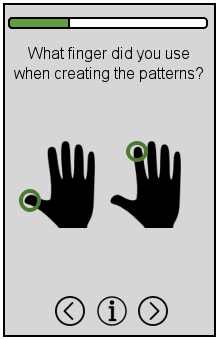
\includegraphics[scale=0.48]{screens/v3/plain/plain2-4.png}
        \label{fig:wireframe11}
      }
      \subfigure[Q5: Reading/Writing orientation]{
        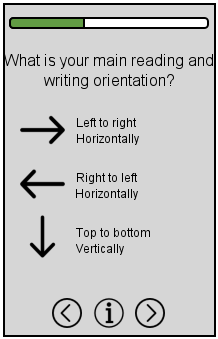
\includegraphics[scale=0.48]{screens/v3/plain/plain2-5.png}
        \label{fig:wireframe12}
      }
      \subfigure[Q6: Gender]{
        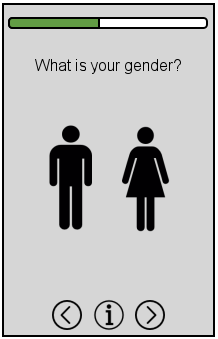
\includegraphics[scale=0.48]{screens/v3/plain/plain2-6.png}
        \label{fig:wireframe13}
      }
    \end{figure}

    When collecting demographics, it is important to know the age of the respondents. It is not known if it will give any results that can be shown to be statistically significant, but it is desired to be able to have a diversity in the age of the respondents. There might be some difference in the risk awareness, or the experience with mobile phones. The age is not grouped into different interval because it is hard to predict reasonable age interval of the sample (Figure~\ref{fig:wireframe14}). The nationality is important to have so it is possible to see how the data is represented on the map. When making statistical tests, it is important to be able to reason about its representation worldwide, or if the results only statistical significant for some part of the world. It is desired to collect data from different nationalities. The respondents selects their nationality from a list. The list might be quite long. To make it easier for the respondents to answer it is possible to map their browser language to their nationality and put them on top of the list. Many respondents might use English as their preferred browser language, then it is not very easy to list specific nationalities on the top of the list. The JavaScript code is illustrated in Listing~\ref{list:language} and the wireframe is illustrated in Figure~\ref{fig:wireframe15}. 

    \medskip
    \begin{lstlisting}[caption=Detecting browser language, label=list:language]
      var browser_language;
      if (navigator.userLanguage) // IE
        browser_language = navigator.userLanguage;
      else if (navigator.language) // FF, Chrome, Safari, Opera
        browser_langauge = navigator.language;
    \end{lstlisting}

    The next wireframe there is a question about whether they have used the Android Unlock Pattern or not (Figure~\ref{fig:wireframe16}). This information can be used to compare respondents that have used the scheme before and those who have not. 

    \begin{figure}[H]
      \ContinuedFloat
      \subfigure[Q7: Age]{
        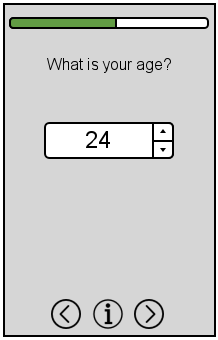
\includegraphics[scale=0.48]{screens/v3/plain/plain2-7.png}
        \label{fig:wireframe14}
      }
      \subfigure[Q8: Nationality]{
        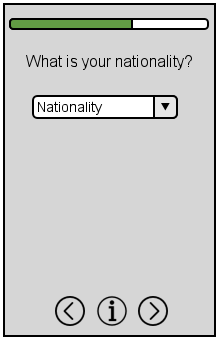
\includegraphics[scale=0.48]{screens/v3/plain/plain2-8.png}
        \label{fig:wireframe15}
      }
      \subfigure[Q9: Android Unlock Pattern experience]{
        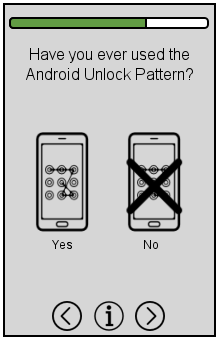
\includegraphics[scale=0.48]{screens/v3/plain/plain2-9.png}
        \label{fig:wireframe16}
      }
    \end{figure}

    Figure~\ref{fig:wireframe17} is asking if the respondents use a screen lock, and if they do, they are redirected to Figure~\ref{fig:wireframe18}. If not, they are directly directed to Figure~\ref{wireframe19}. Figure~\ref{fig:wireframe19} is asking about the mobile Operating System (abbreviated OS) on the mobile used for answering the questionnaire. This is a tricky question to ask because there might be many people that don't know what an operating system is. There are different ways to collect the operating system of the mobile used:

      \begin{enumerate}
        \item You can detect the OS without asking.
        \item You can explicitly ask for the mobile OS and show different icons associated to the mobile operating system (like the apple for iOS and the Droid for Android). 
        \item Combine detection and asking. 
      \end{enumerate}

    The first alternative is not an appropriate way to collect data because I do not want to gather information that the respondents do not know that is collected. The second option is to illustrate the different icons associated with the different mobile operating system. The problem is that the respondent might not know what their mobile operating system is, or they simply don't know what an operating system is. The last option is to detect the mobile OS and then ask the respondent if the detected mobile OS is the mobile OS on their smartphone. It is added an option to answer ``I don't know'' in the case if the respondents feel uncertain. The question is formulated as a generic question: ``is you mobile operating system `detected system' ''. It looks like all participants gets the same question, and the respondents do not get the feeling that the questionnaire is doing something they do not have control over. If the respondent is using an iPhone, the mobile OS can be detected by using JavaScript as described in Listing~\ref{list:mobileOS}.

    \medskip
    \begin{lstlisting}[caption=Detecting mobile OS, label=list:mobileOS]
      var mobileOS;
      if (navigator.userAgent.match(/iPhone/i)){
        mobileOS = 'iOS';
      }
    \end{lstlisting}

    \begin{figure}[H]
      \ContinuedFloat
      \subfigure[Q10: Screen lock usage]{
        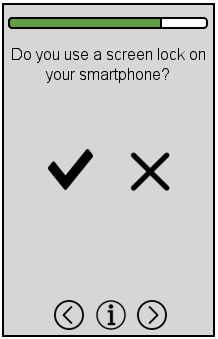
\includegraphics[scale=0.48]{screens/v3/plain/plain2-10.png}
        \label{fig:wireframe17}
      }
      \subfigure[Q11: Selected screen lock]{
        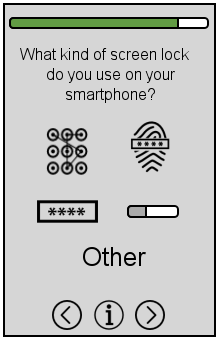
\includegraphics[scale=0.48]{screens/v3/plain/plain2-11.png}
        \label{fig:wireframe18}
      }
       \subfigure[Q12: Mobile OS]{
        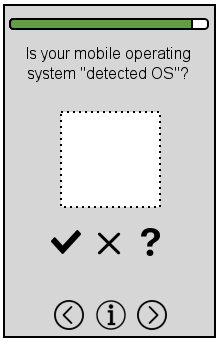
\includegraphics[scale=0.48]{screens/v3/plain/plain2-12.png}
        \label{fig:wireframe19}
      }
    \end{figure}

    The last question is about the respondents experience with IT and security (Figure~\ref{fig:wireframe20}). This question is asked because it is desired to see if people with experience with IT and Security makes different patterns than other respondents. If there is a statistically significant difference, it might introduce bias because they do not represent the whole population. Because of their experience with IT and Security, they might create patterns that are harder to guess. It is also known that people with an interest in security might have a higher interest in participating. The last wireframe (Figure~\ref{fig:wireframe21}) is just a message showing my gratitude to the respondent for using their time to helping by answering the questionnaire. It is here important to provide the same contact information if the respondents have any questions or interest in the study. There might be some respondents that are interested in the results and want to know where they can get the results. 

    \begin{figure}[H]
      \centering
      \ContinuedFloat
      \subfigure[Q13: Experience with IT and security]{
        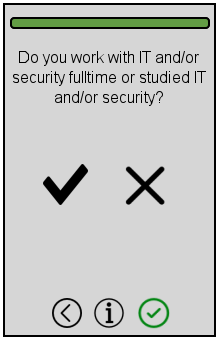
\includegraphics[scale=0.48]{screens/v3/plain/plain2-13.png}
        \label{fig:wireframe20}
      }
      \subfigure[Questionnaire completed]{
        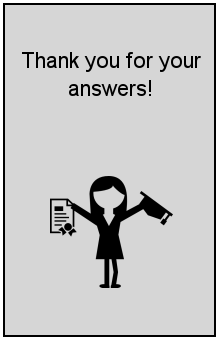
\includegraphics[scale=0.48]{screens/v3/plain/plain2-14.png}
        \label{fig:wireframe21}
      }
      \caption{Wireframes}
    \end{figure}

  \subsection{Pre-test and Pilot}\label{sec:pretest}
    When the questionnaire is ready, I need to perform a questionnaire to evaluate several aspects. First, I need to figure out if the respondents understand the questions stated in the questionnaire. This can cause a lot of bias in the data if the questions asked are ambiguous. Second, the time needed for completion of the questionnaire can not be too long. If the questionnaire takes too long to complete, there is less likely that people want to spend their time completing the questionnaire. It is stated that I need a sample size of 1000 for getting representative results for the analysis. At the same time, there is needed a lot of data to be able to make see patterns in the data. Therefore, it needs to be a balance between questions and data collected, and time of completion. 

    There is a need to do some quality testing before distributing the questionnaire over the Internet. A pen and paper test will be tested to check the wording of the questions as well as getting feedback of the amount of information that is asked for. It is also interesting to ask questions about the ethical aspects of the data collection. If some of the test persons feels that their privacy is leaked by answering the questionnaire, the questions might needs to be evaluated for the final questionnaire. 
    This test will also be conducted in the following spring when the system for data collection is up and running. 

    \todo{En test for tid og en test for ikoner}

  \subsection{Validity and Reliability}\label{sec:validityandreliability}

    {\bf Content validity}

    {\bf Construct validity}

    {\bf Reliability}